\documentclass[11pt]{article}
\usepackage{graphicx}
\usepackage{float}
\usepackage{amsmath}
\usepackage{amsfonts}
\usepackage[brazilian]{babel}
\usepackage[utf8]{inputenc}
\usepackage[T1]{fontenc}

%macros
\newcommand{\fromeng}[1]{\footnote{do inglês: \textit{#1}}}
\newcommand{\tit}[1]{\textit{#1}}
\newcommand{\tbf}[1]{\textbf{#1}}
\newcommand{\ttt}[1]{\texttt{#1}}

\begin{document}

\title{MC833 - Tarefa 6}
\author{Erik de Godoy Perillo - RA: 135582}
\maketitle

\begin{enumerate}

\item --
\begin{itemize}
	\item \ttt{ssize\_t \tbf{recvfrom}(int sockfd, void* buf, size\_t len, 
		int flags, struct sockaddr* src\_addr, socklen\_t *addrlen)}

		Essa função pode ser usada para receber mensagens pela rede por 
		protocolos sem conexão. Por \ttt{sockfd} especifica-se o \tit{socket}
		do sistema operacional a se ``ouvir'' na espera de uma nova mensagem,
		que é guardada em \ttt{buf} e tem o tamanho máximo especificado por
		\ttt{len}. \ttt{flags} pode ser usado para especificar opções sobre
		o comportamento da função, como setá-la para \tit{blocking/nonblocking},
		por exemplo. Se não forem \ttt{NULL}, \ttt{src\_addr} e \ttt{addrlen}
		são preenchidos com o endereço de quem enviou a mensagem e o tamanho
		da estrutura que representa o endereço, respectivamente.
		O valor retornado vai ser o número de \tit{bytes} lidos em caso de 
		sucesso ou -1 caso contrário.

	\item \ttt{ssize\_t sendto(int sockfd, const void* buf, size\_t len, 
		int flags, const struct sockaddr* dest\_addr, socklen\_t addrlen)}

		A contraparte de \ttt{recvfrom}. Pode ser usada para mandar mensagens
		pela rede por protocolos sem conexão. Por \ttt{sockfd} especifica-se
		o \tit{socket} do sistema operacional a se usar para mandar a mensagem,
		que é especificada por \ttt{buf} e tem tamanho em \tit{bytes} dado
		por \ttt{len}. Por \ttt{flags} pode-se configurar algumas partes do 
		comportamento da função, como setar para \tit{blocking/nonblocking}.
		O endereço destino da mensagem é especificado por \ttt{dest\_addr}
		e seu tamanho é especificado em \ttt{addrlen}. Em sucesso, retorna o 
		número de bytes enviados. Se falhar, retorna -1.
		
\end{itemize}

\item O servidor e cliente foram implementados. Uma demonstração é ilustrada
abaixo, onde o cliente feito e o programa \ttt{nc} são usados ao mesmo tempo
para mandar mensagens ao servidor, que as manda de volta para os respectivos
clientes:
\begin{figure}[H]
	\centering
	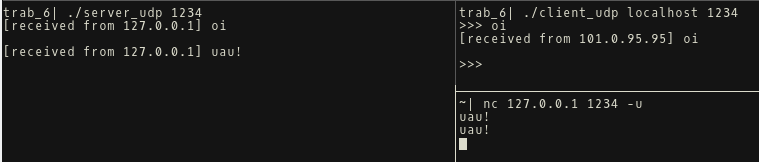
\includegraphics[width=1.0\linewidth]{img/teste.png}
\end{figure}

\item A principal diferença entre o protocolo UDP e o TCP é que o primeiro
não é conectado a conexão, enquanto o outro é. Assim, UDP é efêmero no sentido
que só existe a troca da mensagem entre um \tit{host} e outro, enquanto que no
TCP uma conexão é mantida até que não se queira/possa mais trocar mensagens.
O UDP usa o método conhecido como \tit{best effort}, isto é: 
tenta-se enviar a mensagem ao destinatário,
mas nada é garantido. Em TCP, há diversas medidas que asseguram que a mensagem
foi enviada ao destinatário, como mensagens de confirmação etc.
Em TCP também garante-se que os pacotes chegam em ordem, em UDP, não.
Por esses motivos e outros, o TCP é naturalmente mais complexo que o UDP. 
Tende-se a usar o TCP em casos em que a) pode-se pagar pelo \tit{overhead} e
b) é importante que todas as mensagens cheguem e o façam em ordem. UDP é mais
usado em casos onde não é terrível a perda de alguns pacotes e um custo
computacional baixo é apreciado/necessário.

\item O servidor foi modificado para mostrar a porta de quem o envia as 
	mensagens. Assim, por meio do uso do \ttt{nc}, pôde-se enviar uma 
	mensagem para o cliente, a qual ele aceitou sem problema algum.
\begin{figure}[H]
	\centering
	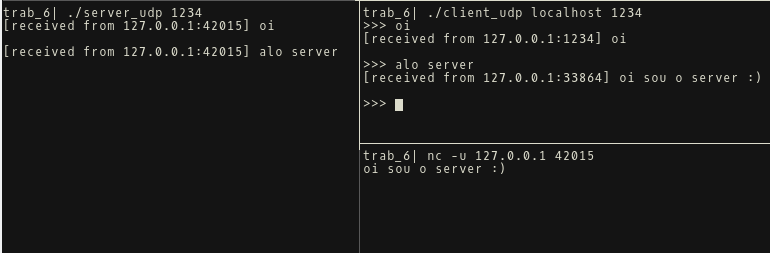
\includegraphics[width=1.0\linewidth]{img/malicia.png}
\end{figure}

\item O cliente foi modificado para checar o endereço/porta de quem o mandou
	a mensagem. Se eles forem de algum modo diferentes dos especificados como
	sendo do servidor, a mensagem é ignorada e um aviso é mostrado, como
	ilustrado abaixo:
\begin{figure}[H]
	\centering
	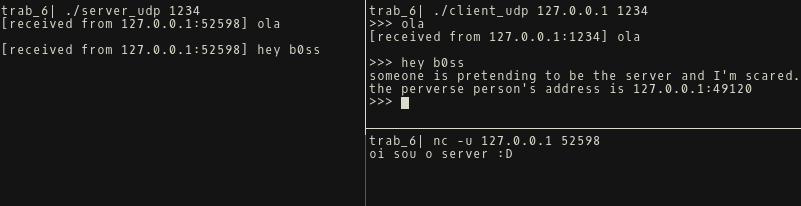
\includegraphics[width=1.0\linewidth]{img/tepeguei.png}
\end{figure}

\end{enumerate}

\end{document}
